% Evaluation protocols: (a) end-of-timeline, (b) continual probing, (c) live simulation.
% Standalone so it compiles on its own (e.g. `tectonic protocols.tex`); include protocols.pdf in a figure*.
\documentclass[tikz,border=3pt]{standalone}
\usepackage{newtxtext,newtxmath}
\usetikzlibrary{arrows.meta,positioning,calc,decorations.pathreplacing}
\definecolor{acc}{RGB}{0,102,153}

\tikzset{
  >={Stealth[length=2mm]},
  every node/.style={font=\footnotesize},
  blk/.style={draw, rounded corners=1.5pt, minimum height=8mm, minimum width=17mm, align=center, inner sep=2pt},
  mem/.style={blk, fill=acc!12, draw=acc, thick},
  sess/.style={draw, minimum width=5mm, minimum height=5.5mm, inner sep=0pt, fill=black!6},
  lab/.style={font=\scriptsize\itshape, text=black!70, inner sep=1.5pt},
  panel/.style={font=\small\bfseries, anchor=west},
  rd/.style={->, acc, thick},
}

\begin{document}
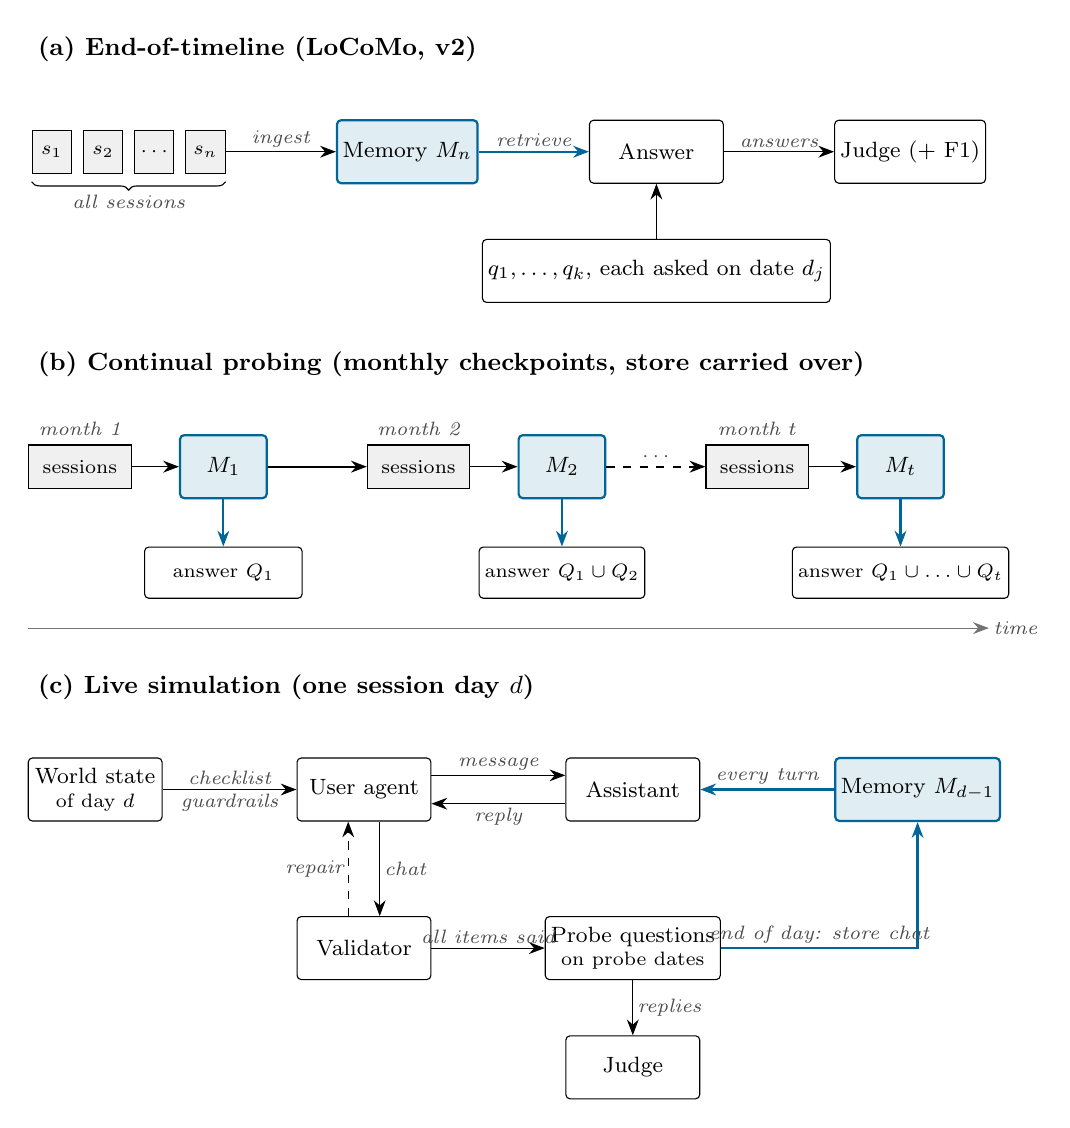
\begin{tikzpicture}

% ---------------------------------------------------------------- (a) end of timeline
\node[panel] at (0,1.3) {(a) End-of-timeline (LoCoMo, \textsc{v2})};
\foreach \i/\t in {0/$s_1$,1/$s_2$,2/$\cdots$,3/$s_n$}
  \node[sess] (a\i) at (0.3+\i*0.65,0) {\scriptsize\t};
\draw[decorate, decoration={brace, mirror, amplitude=3pt}]
  ($(a0.south west)+(0,-0.1)$) -- ($(a3.south east)+(0,-0.1)$) node[midway, below=3pt, lab] {all sessions};
\node[mem, right=14mm of a3] (am) {Memory $M_n$};
\draw[->] (a3) -- node[above, lab] {ingest} (am);
\node[blk, right=14mm of am] (aa) {Answer};
\draw[rd] (am) -- node[above, lab] {retrieve} (aa);
\node[blk, below=7mm of aa, minimum width=30mm] (aq) {$q_1,\dots,q_k$, each asked on date $d_j$};
\draw[->] (aq) -- (aa);
\node[blk, right=14mm of aa] (aj) {Judge (+ F1)};
\draw[->] (aa) -- node[above, lab] {answers} (aj);

% ---------------------------------------------------------------- (b) continual probing
\begin{scope}[yshift=-4.0cm]
\node[panel] at (0,1.3) {(b) Continual probing (monthly checkpoints, store carried over)};
\foreach \m/\x/\lbl/\qs in {1/0/month 1/$Q_1$, 2/4.3/month 2/$Q_1\cup Q_2$, 3/8.6/month $t$/$Q_1\cup\dots\cup Q_t$} {
  \node[sess, minimum width=13mm, anchor=west] (bs\m) at (\x,0) {\scriptsize sessions};
  \node[lab, above=0.5mm of bs\m] {\lbl};
  \node[mem, right=6mm of bs\m, minimum width=11mm] (bm\m) {};
  \draw[->] (bs\m) -- (bm\m);
  \node[blk, below=6mm of bm\m, minimum width=20mm, minimum height=6.5mm] (bq\m) {\scriptsize answer \qs};
  \draw[rd] (bm\m) -- (bq\m);
}
\node at (bm1) {$M_1$}; \node at (bm2) {$M_2$}; \node at (bm3) {$M_t$};
\draw[->, thick] (bm1.east) -- (bs2.west);
\draw[->, thick, dashed] (bm2.east) -- node[above, lab] {$\cdots$} (bs3.west);
\draw[->, black!55] (0,-2.05) -- (12.2,-2.05) node[right, lab] {time};
\end{scope}

% ---------------------------------------------------------------- (c) live simulation
\begin{scope}[yshift=-8.1cm]
\node[panel] at (0,1.3) {(c) Live simulation (one session day $d$)};
\node[blk] (cw) at (0.85,0) {World state\\[-1pt]\scriptsize of day $d$};
\node[blk, right=17mm of cw] (cu) {User agent};
\node[blk, right=17mm of cu] (ca) {Assistant};
\node[mem, right=17mm of ca] (cm) {Memory $M_{d-1}$};
\draw[->] (cw) -- node[above, lab] {checklist} node[below, lab] {guardrails} (cu);
\draw[->] ([yshift=1.8mm]cu.east) -- node[above, lab] {message} ([yshift=1.8mm]ca.west);
\draw[->] ([yshift=-1.8mm]ca.west) -- node[below, lab] {reply} ([yshift=-1.8mm]cu.west -| cu.east);
\draw[rd] (cm) -- node[above, lab] {every turn} (ca);

\node[blk, below=12mm of cu] (cv) {Validator};
\draw[->] ([xshift=2mm]cu.south) -- node[right, lab] {chat} ([xshift=2mm]cv.north);
\draw[->, dashed] ([xshift=-2mm]cv.north) -- node[left, lab] {repair} ([xshift=-2mm]cu.south);
\node[blk, below=12mm of ca] (cp) {Probe questions\\[-1pt]\scriptsize on probe dates};
\draw[->] (cv) -- node[above, lab] {all items said} (cp);
\node[blk, below=7mm of cp] (cj) {Judge};
\draw[->] (cp) -- node[right, lab] {replies} (cj);
\draw[rd] (cp.east) -| node[pos=0.25, above, lab] {end of day: store chat} (cm.south);
\end{scope}

\end{tikzpicture}
\end{document}
